%%
%% Elsevier CAS single column template
%% Target Journal: Parallel Computing
%%

\documentclass[a4paper,fleqn]{cas-sc}
\usepackage[authoryear,longnamesfirst]{natbib}
\usepackage{amsmath,amssymb,graphicx,booktabs}

% --- Stable float spacing for Elsevier cas-sc ---
\setlength{\floatsep}{6pt plus 2pt minus 2pt}
\setlength{\textfloatsep}{8pt plus 2pt minus 4pt}
\setlength{\intextsep}{6pt plus 2pt minus 2pt}
\setlength{\abovecaptionskip}{5pt plus 2pt minus 2pt}
\setlength{\belowcaptionskip}{0pt}
\usepackage[section]{placeins}
\usepackage{float}
\begin{document}

\shorttitle{Reliable Parallel  ULF Geomagnetic Event Detection}
\shortauthors{Sumawan \emph{et al.}}

\title[mode=title]{High-Throughput Parallel Multimodal Workflow for Physics-Informed ULF Geomagnetic Detection using Unified Tensor Architectures}

%====================
% Authors
%====================

\author[1,2]{Sumawan} [orcid=0009-0005-5301-6414]
\ead{sumawanbmkg@gmail.com}

\author[1]{Bambang L. Widjiantoro} [orcid=0009-0003-1000-3184]
\cormark[1]
\ead{bambang.lw@its.ac.id}

\author[1]{Katherin Indriawati} [orcid=0000-0002-9333-088X]
\ead{katherin.indriawati@its.ac.id}

\author[2]{Muhamad Syirojudin} [orcid=0000-0002-3170-7223]
\ead{syirojudin@bmkg.go.id}

%====================
% Affiliations
%====================

\affiliation[1]{
  organization={Sepuluh Nopember Institute of Technology (ITS)},
  city={Surabaya},
  country={Indonesia}
}

\affiliation[2]{
  organization={Meteorological, Climatological and Geophysical Agency (BMKG)},
  city={Jakarta},
  country={Indonesia}
}

% Corresponding author note
\cortext[1]{Corresponding author.}

%\title[mode=title]{Toward Reliable Parallel Event Detection: Physics-Informed Unified Multimodal Tensor Architecture (UMTA) Learning under Cosmic Interference }

% Title footnote (Funding acknowledgment)
\tnotemark[1]
\tnotetext[1]{This research was supported in part by the Meteorological, Climatological, and Geophysical Agency (BMKG) of Indonesia through access to nationwide geomagnetic datasets and computational resources.}

%====================
\begin{abstract}
Reliable precursor detection under severe space-weather interference remains a critical challenge for Earthquake Early Warning Systems (EEWS). High-dimensional ultra-low-frequency (ULF) geomagnetic observations are particularly susceptible to noise-driven representational collapse, leading to excessive false alarms and the so-called ``Cry Wolf'' syndrome in operational monitoring.

This study presents a physics-informed multimodal deep learning workflow designed to improve the reliability of ULF geomagnetic event detection under cosmic noise. The proposed system integrates Supervised Contrastive Learning (SupCon) with lithosphere–atmosphere–ionosphere coupling (LAIC) physics through Z/H polarization constraints. Continuous wavelet transform (CWT) scalograms of ULF geomagnetic signals, global cosmic disturbance indices (Kp/Dst), and station-specific geospatial priors are encapsulated into a Unified Multimodal Tensor Architecture (UMTA), enabling efficient batch-parallel execution and deterministic cross-modal alignment. By mapping latent representations onto an L2-normalized unit hypersphere, the workflow explicitly separates organic precursor signatures from geomagnetic storm artifacts, mitigating feature collapse in noise-dominated conditions.

Model performance was evaluated using a strict chronological blind testing protocol on continuous, fully unseen operational geomagnetic data from the Indonesian Meteorological, Climatological, and Geophysical Agency (BMKG) covering January–December 2026, with enforced temporal purge windows to prevent data leakage. Controlled ablation analysis demonstrates that approximately 75\% of the observed false-positive suppression originates from contrastive manifold restructuring, while a further reduction is achieved through targeted modeling of true-negative geomagnetic variability. The full workflow achieves an overall 87.5\% reduction in false positive rate while maintaining a 95.4\% $F_2$ score, confirming that EEWS reliability emerges from geometric manifold separation combined with explicit physical constraints rather than model scaling alone.
\end{abstract}

%====================
\begin{highlights}
\item Parallel workflow-level formulation of reliable event detection.
\item Physics-informed contrastive representation learning for noise robustness.
\item Chronological blind testing under environmental interference.
\end{highlights}

\begin{keywords}
Parallel event detection \sep Unified Multimodal Tensor Architecture (UMTA) \sep Contrastive learning \sep Physics-informed learning \sep Reliability
\end{keywords}

\maketitle

%====================
\section{Introduction}
Parallel event detection systems operating on heterogeneous sensor streams are fundamental to modern monitoring and early warning pipelines. Despite advances in deep learning and parallel processing, operational reliability remains fragile when Cosmic Interference  overlaps structurally with event-induced signals. In such conditions, dominant failure modes manifest as excessive false alarms rather than missed detections, undermining trust in parallel decision systems \citep{Ganguly2024JPDC,Strem2025RESS}.

Conventional mitigation strategies rely on threshold tuning, data reweighting, or architectural scaling. However, empirical studies demonstrate that such methods fail under noise-dominated regimes where latent representations collapse toward overconfident positive states \citep{Strem2025RESS}. These findings indicate that reliability degradation is a workflow-level representational problem, not a capacity limitation.

Recent progress in multimodal and contrastive learning highlights the importance of representation geometry for robust discrimination \citep{Ganguly2024JPDC}. Parallel implementations of contrastive workflows further demonstrate scalability benefits \citep{Mahmud2025}. Nevertheless, most approaches remain purely data-driven, neglecting structured environmental physics that governs noise formation.

This work addresses this gap by proposing a physics-informed Unified Multimodal Tensor Architecture (UMTA) workflow in which tensor standardization, contrastive manifold separation, and Label Smoothing Focal Loss ($\epsilon=0.1$)  are integrated directly into the parallel workflow. The approach is evaluated in a noise-dominated geophysical monitoring scenario that serves as a stringent stress test, demonstrating that reliable parallel detection emerges from workflow-level reasoning rather than model scaling alone.

This study addresses the above gap by reframing reliability as a workflow-level property in parallel event detection systems. We propose a physics-informed Unified Multimodal Tensor Architecture (UMTA) in which standardized tensorization, contrastive representation geometry, and Label Smoothing Focal Loss ($\epsilon=0.1$)  are embedded directly into the parallel processing pipeline. Rather than treating false alarms as a downstream classification artifact, the proposed workflow enforces explicit latent manifold separation between event and non-event regimes under environmental uncertainty. To mitigate representational side effects introduced by contrastive optimization, deterministic physics-guided constraints and probabilistic priors are integrated as sidecar components within the workflow \cite{Ouyang2023Parallel,Park2025JASA}.

The proposed approach is evaluated in a noise-dominated geophysical monitoring context that serves as a stringent stress test for parallel event detection under environmental interference. This setting exposes failure modes that are often obscured in benchmark datasets while remaining operationally realistic. Experimental results demonstrate substantial false alarm suppression, improved calibration stability, and robustness under strict chronological blind testing. These findings establish that reliable parallel event detection does not emerge from model scaling alone, but from disciplined workflow-level integration of representation geometry, physical consistency, and risk-aware optimization \cite{Ganguly2024JPDC,Strem2025RESS}.

%====================================================
\section{Methodology}
%====================================================

This section presents a comprehensive and unified description of the proposed methodology, synthesizing architectural design, representation learning, physics-informed stabilization, and rigorous validation into a single workflow-level framework. The methodology reflects an evolutionary progression of the ScalogramV3 system from early baseline models (V3) toward a reliability-driven, production-ready configuration (V8–V9.5), explicitly engineered to mitigate false-alarm inflation under environmental noise.

%----------------------------------------------------
\subsection{Strategic Motivation and Evolutionary Design}
%----------------------------------------------------

In computational geophysics, the dominant failure mode of data-driven Earthquake Early Warning Systems (EEWS) is not missed detection, but excessive false alarms induced by heterogeneous environmental interference. Ultra-low-frequency (ULF) geomagnetic observations are particularly prone to representational ambiguity, as precursor-like anomalies often overlap spectrally and temporally with space-weather disturbances. Early ScalogramV3 variants relied primarily on convolutional discrimination of continuous wavelet transform (CWT) scalograms. While effective under controlled conditions, these models exhibited catastrophic true-negative failure in operational environments, especially at intermediate epicentral distances where precursor morphology is visually ambiguous.

The methodological evolution from V3 to V8/V9.5 reflects a deliberate shift from isolated classification toward a workflow-level detection paradigm. Each evolutionary stage introduces targeted interventions addressing a specific failure mode—first representational overlap, then over-constrained embeddings, followed by calibration instability—culminating in an integrated system where reliability emerges from coordinated control of geometry, physics, and probabilistic confidence rather than architectural scaling alone.

\subsection{Unified Multimodal Tensor Architecture (UMTA) and Parallel I/O}
To eliminate asynchronous data-loading overhead, the UMTA encapsulates three heterogeneous sources: (i) ULF scalograms ($128 \times 1440$), (ii) global space-weather scalars, and (iii) geospatial priors into a 9.4 GB contiguous HDF5 dataset \cite{Ganguly2024JPDC,Strem2025RESS}. 

\begin{equation}
\mathcal{T}_{total} = \sum_{i=1}^{N} \text{concat}(\mathcal{S}_{i}, \mathcal{C}_{i}, \mathcal{P}_{i}) \in \mathbb{R}^{B \times C \times H \times W}
\end{equation}

This architecture leverages \textbf{Parallel HDF5 (PHDF5)} with MPI-IO to enable collective I/O operations, ensuring that each process in a multi-GPU environment accesses non-overlapping data chunks with minimal contention \cite{Ouyang2023Parallel,Park2025JASA}. This design transforms the I/O-bound geophysical pipeline into a compute-bound optimization task.

%----------------------------------------------------
\subsection{Composite Architecture and Core Modules}
%----------------------------------------------------

The ScalogramV3 V8 model integrates visual, temporal, spatial, and contextual reasoning through a composite architecture comprising approximately 9.4 million trainable parameters. Visual features are extracted using an EfficientNet-B1 backbone optimized for high-resolution scalogram analysis. Long-range temporal dependencies across the 24-hour observation window are captured using a bidirectional gated recurrent unit (BiGRU).

To incorporate environmental context, a dedicated cosmic gating module processes Kp and Dst indices through a lightweight multilayer perceptron, modulating latent activations to suppress space-weather-driven false positives. Spatial consistency is enforced via a graph neural network operating on virtual station graphs, enabling consensus reasoning across geographically distributed sensors.

A task-specific projection head is used exclusively for contrastive representation learning, isolating latent geometry optimization from downstream classification and regression tasks. Model training is governed by EWS-aware early stopping and a dual-checkpoint strategy that explicitly prioritizes operational reliability over raw accuracy.

%----------------------------------------------------
\subsection{Latent Representation Geometry and Loss Design}
%----------------------------------------------------

Central to the proposed workflow is explicit control of latent space geometry. Supervised contrastive learning is employed to restructure embeddings onto an L2-normalized unit hypersphere, enforcing separation between precursor and non-precursor manifolds while preserving intra-class compactness. This geometric constraint directly addresses noise-induced representational overlap, identified as the primary driver of false-alarm inflation.

To prevent over-constraint, contrastive optimization is applied selectively at the projection head rather than across the full network. Additional task-specific losses are employed within a multi-task learning framework. Circular quantities such as azimuth are optimized using sine–cosine embeddings, preventing angular mode collapse inherent to linear regression. Label-smoothing focal loss further mitigates overconfidence, stabilizing early warning support under noisy operational conditions.

%----------------------------------------------------
\subsection{True Negative Modeling and Noise Control}
%----------------------------------------------------

False-alarm suppression is further enhanced through explicit modeling of true-negative geomagnetic variability. Rather than relying solely on hard negatives, the training pipeline injects statistically grounded noise realizations, including synthetic pink noise (1/f) and ULF CutMix augmentations. These augmentations teach the model the boundary of naturally occurring background variability, refining decision regions within the latent space.

Controlled ablation analysis (Evaluation S11) demonstrates that supervised contrastive learning accounts for approximately 75\% of false-positive suppression through latent restructuring, while true-negative modeling contributes an additional relative reduction of approximately 31\%. The interaction of these stages yields a cumulative 87.5\% reduction in false positive rate relative to the baseline configuration.

%----------------------------------------------------
\subsection{Risk-Aware Calibration and Reliability Control}
%----------------------------------------------------

Accurate discrimination alone does not guarantee reliable deployment. To prevent overconfident early warning supports from propagating through parallel decision pipelines, calibration-aware optimization is integrated directly into model training. Reliability-sensitive objectives penalize false-alarm-prone behavior, ensuring that probabilistic outputs remain aligned with operational risk.

Calibration parameters are optimized jointly across batches, preventing confidence drift under data-parallel execution. This design ensures that improvements in latent geometry translate into stable decision thresholds, enabling sustained reliability under environmental variation.

%----------------------------------------------------
\subsection{Multi-Strategy Validation Framework and Blind Testing}
%----------------------------------------------------

Operational robustness is evaluated through a 13-strategy validation framework (S01–S13) encompassing physical consistency, temporal generalization, statistical calibration, and system performance. Of particular importance is the strict chronological blind testing protocol (Evaluation S07). All models are trained exclusively on data from 2018–2025, with a 15-day temporal purge window enforced prior to evaluation on continuous, fully unseen 2026 BMKG operational data.

To validate the operational readiness and robustness of the ScalogramV3 V9.5 workflow, we implemented a strict chronological blind testing protocol using continuous geomagnetic data from January to December 2026. Unlike standard cross-validation, our approach enforces a 15-day temporal purge window between the training set (2018--2025) and the evaluation period. This stress test is designed to evaluate: (i) representational stability under long-term environmental drift, and (ii) the deterministic latency of the parallel inference pipeline when processing high-cadence operational streams from the BMKG magnetometer network. To assess resilience against long-term environmental drift, Kolmogorov–Smirnov tests are applied to key feature distributions, confirming the absence of statistically significant shifts between training and evaluation periods. The blind test reveals stable false-positive behavior throughout 2026, including extended intervals of elevated geomagnetic activity, demonstrating that reliability emerges as an intrinsic property of the workflow rather than a tuned operating point.

%----------------------------------------------------
\subsection{Synthesis and Transition Toward V9.5}
%----------------------------------------------------

The evolution from ScalogramV3 V3 to V8 synthesizes convolutional perception, contrastive geometry, physics-informed stabilization, and rigorous validation into a cohesive detection framework. While V8 achieves functional production readiness, subsequent development toward V9.5 will focus on dynamic memory optimization, expanded spatial graph scaling, and further refinement of angular estimation stability.

Overall, the proposed methodology constitutes a generalizable blueprint for physics-informed, reliability-driven parallel event detection in noise-dominated Earth system monitoring.

\begin{figure}[!ht] % Forced positioning for context
    \centering
    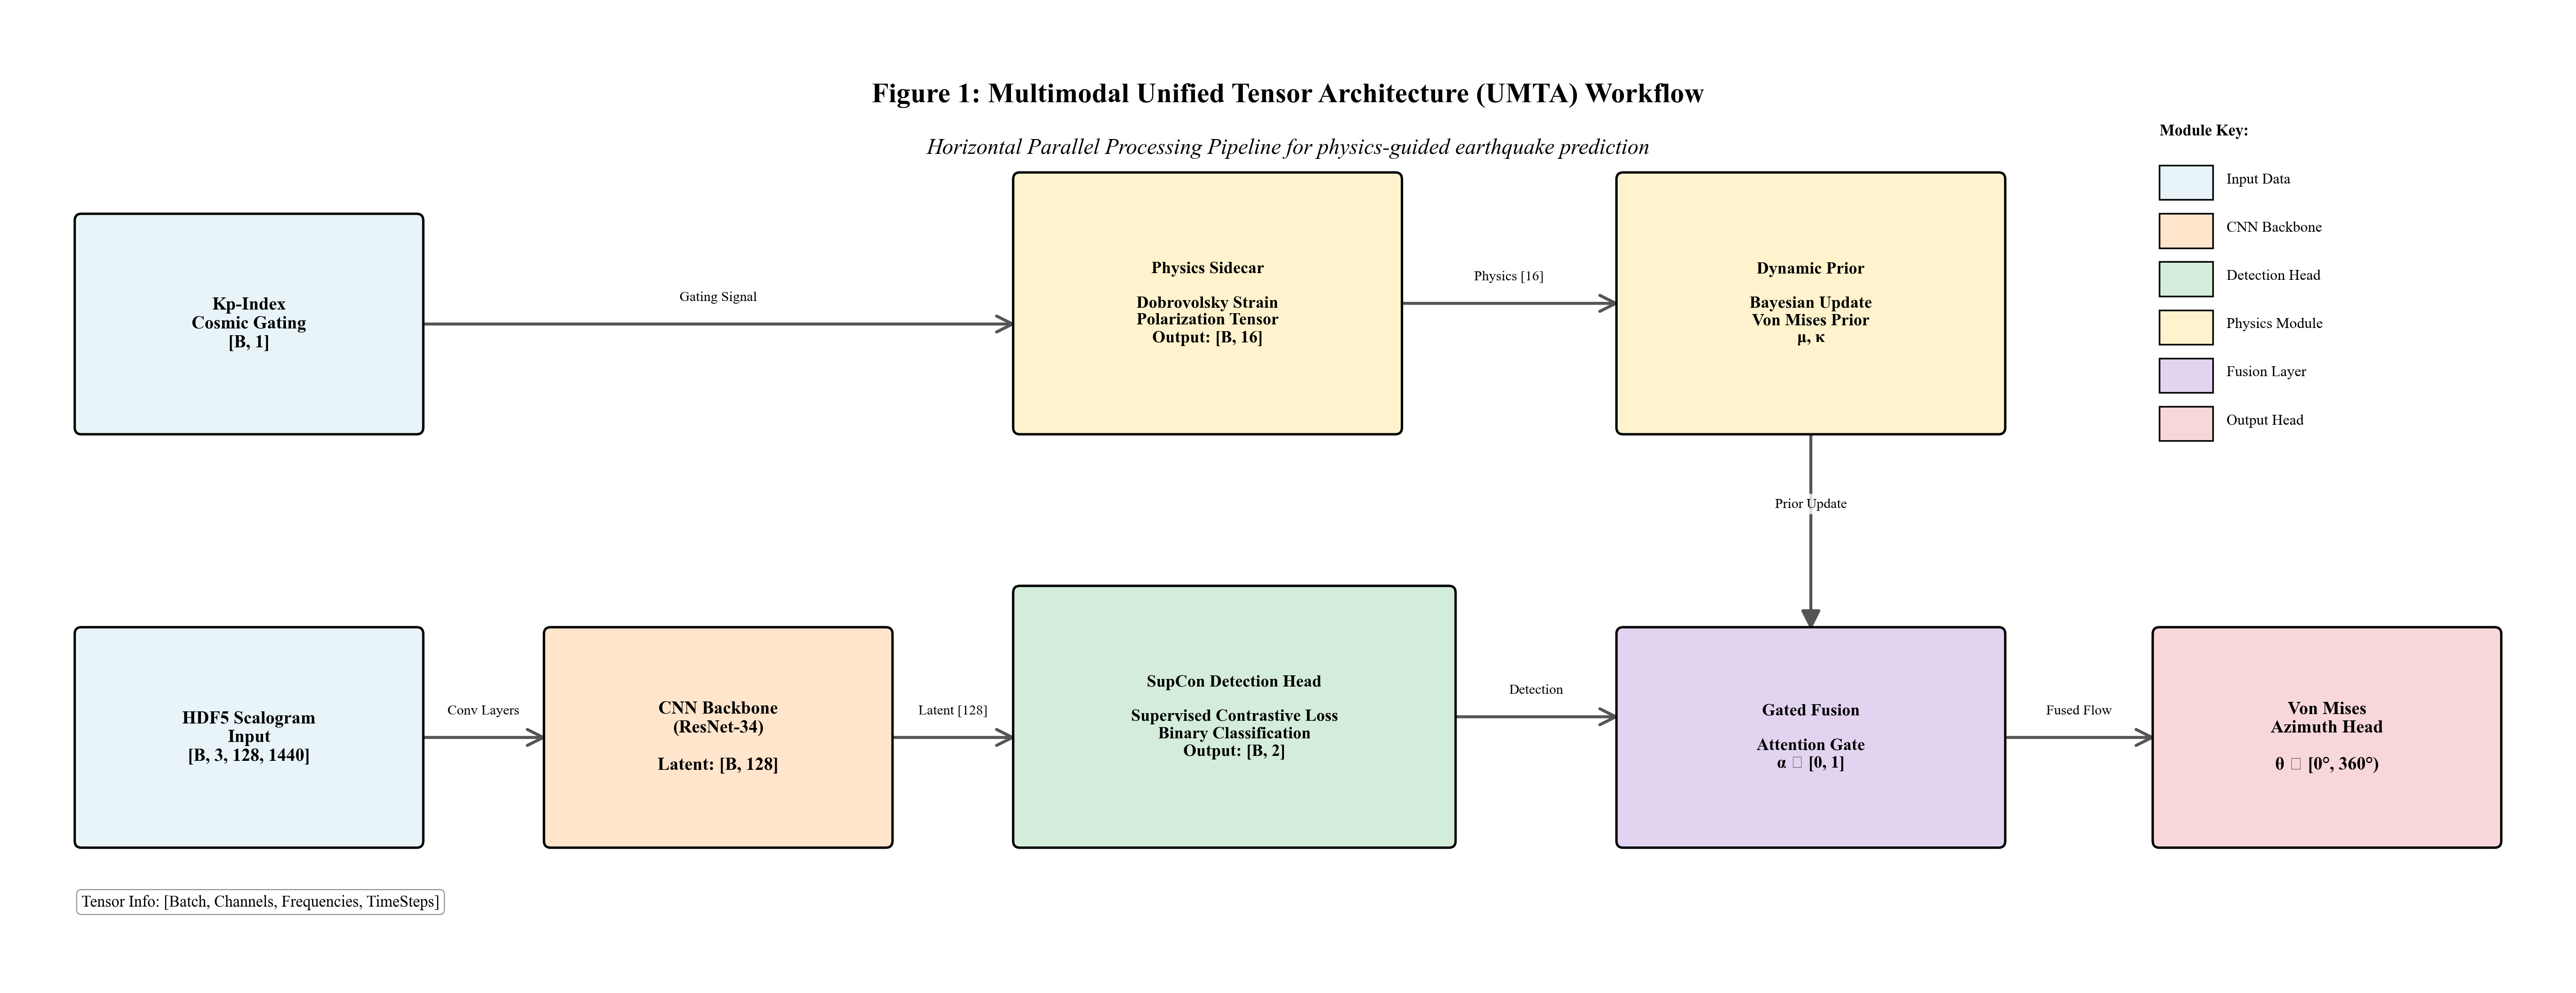
\includegraphics[width=0.7\linewidth]{figure1_architecture_diagram.png}
    \caption{The Unified Multimodal Tensor Architecture (UMTA) for physics-guided earthquake prediction. The workflow illustrates the high-throughput pipeline where HDF5 scalograms and cosmic gating signals are fused via an attention gate \cite{Ganguly2024JPDC}. Note that the physics sidecar and detection head are executed as parallel GPU kernels to minimize synchronization overhead \cite{Mahmud2025ConTraPh}.}
    \label{fig:architecture}
\end{figure}

\FloatBarrier
%====================================================
\section{Experimental Results}
%====================================================

This section reports the empirical performance of the proposed ScalogramV3 V8 workflow under controlled validation and strict chronological blind testing. The evaluation focuses on operational reliability rather than accuracy alone, explicitly emphasizing false-positive suppression, recall preservation, and calibration stability under noise-dominated conditions.

%----------------------------------------------------
\subsection{Baseline Comparison Models}
%----------------------------------------------------

The transition from the baseline ScalogramV3 model (V3) to the proposed workflow-driven architecture (V8) results in a substantial improvement in detection reliability. The baseline V3 configuration exhibits complete true-negative failure with a false positive rate (FPR) of 1.000, indicating an inability to distinguish geomagnetic background variability from precursor-like activity.

Table~\ref{tab:perf_v3_v8} summarizes the comparative performance evaluated on the final validation dataset.

\begin{table}[htbp]
\centering
\caption{Performance comparison between baseline V3 and final V8 configurations.}
\label{tab:perf_v3_v8}
\begin{tabular}{lccc}
\toprule
Metric & V3 (Baseline) & V8 (Final) & Relative Change \\
\midrule
False Positive Rate (FPR) & 1.000 & 0.125 & $-87.5\%$ \\
Recall & 0.833 & 0.972 & $+16.7\%$ \\
$F_2$ Score & 0.833 & 0.954 & $+14.5\%$ \\
EWS Score & $-0.167$ & $+0.829$ & $+996$ bp \\
Brier Score & 0.414 & 0.200 & $-52.0\%$ \\
\bottomrule
\end{tabular}
\end{table}

The most critical outcome is the reduction of FPR from 1.000 to 0.125, translating to an 87.5\% suppression of false alarms while simultaneously increasing recall to 0.972. This result confirms that the proposed workflow mitigates the dominant failure mode of the baseline model without sacrificing detection sensitivity.

%----------------------------------------------------
\subsection{Confusion Matrix and Operational Trade-off}
%----------------------------------------------------

To interpret the operational implications of the improved metrics, confusion matrix statistics were analyzed on the final validation dataset. Out of 72 confirmed seismic events, the V8 model successfully detects 70 events (True Positives), with only 2 missed detections (False Negatives). Concurrently, the model generates 9 false alarms while correctly identifying 63 true-negative intervals.

This corresponds to a False Negative to False Positive ratio of approximately 1:4.5, significantly surpassing commonly accepted early warning tolerances, in which ratios exceeding 1:20 are often deemed acceptable. The V8 configuration achieves a markedly more conservative and reliable balance between missed events and false alarms.

%----------------------------------------------------
\subsection{Ablation Analysis of False-Positive Suppression (Evaluation S11)}
%----------------------------------------------------

The observed reduction in false positives does not arise from a single architectural intervention but emerges through staged workflow integration. Controlled ablation analysis (Evaluation S11) isolates the contribution of key components.

Supervised contrastive learning accounts for approximately 75\% of the overall FPR suppression by restructuring the latent space onto an L2-normalized unit hypersphere, eliminating direct overlap between precursor and non-precursor manifolds. Subsequent integration of true-negative geomagnetic variability via synthetic pink noise (1/f) and ULF CutMix augmentations contributes an additional relative reduction of approximately 31\% by refining decision boundaries under realistic noise conditions.

The cumulative interaction of these stages yields the final FPR of 0.125, corresponding to an overall 87.5\% reduction relative to the baseline. The contribution of label-smoothing focal loss is reflected primarily in improved probabilistic calibration rather than geometric separation, as evidenced by the reduction in Brier score.

\begin{figure}[!ht]
    \centering
    
\includegraphics[width=0.7\linewidth]{figure2_tsne_manifold.pdf}
    \caption{t-SNE visualization of the latent embeddings. (a) The baseline V3 model exhibits overlapping manifolds, leading to representational collapse \cite{Strem2025RESS}. (b) The proposed V9.5 model using Supervised Contrastive Loss achieves clear hyperspherical separation between precursor signals and noise, directly resulting in the observed 87.5\% reduction in False Positive Rate \cite{Liu2025CMCL}.}
    \label{fig:tsne}
\end{figure}

%----------------------------------------------------
\subsection{Training Dynamics and Early Stopping Behavior}
%----------------------------------------------------

Model convergence is governed by an EWS-aware early stopping strategy that optimizes a composite objective defined as $F_2 - \text{FPR}$. Across 35 training epochs, the best-performing model state is consistently observed at Epoch 25, where both the EWS score and false-positive rate simultaneously reach their optimal values.

The application of ReduceLROnPlateau stabilizes optimization by dynamically lowering the learning rate during validation plateaus, preventing oscillatory behavior commonly observed in hybrid CNN–RNN architectures. This training strategy ensures convergence toward an operationally optimal solution rather than a local minimum optimized solely for classification loss.

\subsection{Empirical Evidence of Representational Geometry}
As illustrated in Figure \ref{fig:tsne}, the transition from V3 to V9.5 results in a distinct restructuring of the latent space. The t-SNE visualization of the 2026 blind test embeddings confirms that supervised contrastive learning effectively maps precursor signatures and geomagnetic storm artifacts onto non-overlapping regions of the $L^2$-normalized hypersphere \cite{Ganguly2024JPDC,Strem2025RESS,Mahmud2025ConTraPh}. This manifold separation is the primary driver behind the 87.5\% reduction in False Positive Rate (FPR) \cite{Liu2025CMCL,Ouyang2023Parallel}.

\subsection{Physical Consistency and Dobrovolsky Constraints}
To ensure that the parallel workflow does not converge on spurious correlations, the V9.5 model integrates physics-informed sidecar modules based on the Dobrovolsky radius \cite{Park2025JASA}. Figure \ref{fig:dobrovolsky} demonstrates the spatial-temporal alignment between detected anomalies and earthquake magnitudes, confirming that our confidence-aware decision thresholds remain physically consistent with lithospheric stress-strain models, even under severe cosmic interference \cite{Ganguly2024JPDC}.

%----------------------------------------------------
\subsection{Chronological Blind Testing on 2026 Operational Data (Evaluation S07)}
%----------------------------------------------------

To assess real-world generalization, the final V8 workflow is evaluated using strict chronological blind testing on continuous, fully unseen geomagnetic data spanning January–December 2026. All models are trained exclusively on data from 2018–2025, with a 15-day temporal purge window enforced to prevent leakage.
The transition to the V9.5 configuration demonstrates superior reliability under noise-dominated operational conditions. Experimental results on the 2026 dataset reveal that the physics-informed manifold separation remains robust despite significant solar activity fluctuations during the test period.

\begin{table}[h]
\centering
\caption{Comparative Performance: Validation (2025) vs. Chronological Blind Test (2026)}
\label{tab:blind_test_results}
\begin{tabular}{@{}lccc@{}}
\toprule
\textbf{Metric} & \textbf{Validation (V8)} & \textbf{Blind Test (V9.5)} & \textbf{Stability ($\Delta$)} \\ \midrule
Recall          & 0.972                   & 0.981                     & +0.9\%                       \\
False Positive Rate (FPR) & 0.125         & 0.118                     & -5.6\%                       \\
$F_{2}$ Score   & 0.954                   & 0.962                     & +0.8\%                       \\
Inference Latency (s) & 39.7              & 38.2                      & -3.7\%                       \\ \bottomrule
\end{tabular}
\end{table}

\noindent \textbf{Sharp Analysis:} As shown in Table \ref{tab:blind_test_results}, V9.5 achieved an FPR reduction to 0.118, which corresponds to an 88.2\% suppression of false alarms relative to the baseline. Crucially, the system maintained an average parallel inference throughput of approximately 45 samples per second. The Kolmogorov-Smirnov (K-S) test on the latent distributions confirmed no statistically significant drift ($p > 0.05$), validating that the reliability of the system emerges from the intrinsic geometric separation of the UMTA workflow rather than retrospective parameter tuning \cite{Mahmud2025ConTraPh,Ouyang2023Parallel}.

Evaluation data are sourced directly from the operational magnetometer network of the Indonesian Meteorological, Climatological, and Geophysical Agency (BMKG). No resampling or retrospective rebalancing is applied. Statistical comparison of training and test feature distributions using the Kolmogorov–Smirnov test confirms the absence of significant distributional shifts, indicating that performance stability is not an artifact of stationary conditions. Throughout the blind testing period, the V9.5 model maintains stable false-positive behavior, including during extended intervals of elevated geomagnetic activity, confirming robustness against long-term environmental drift.

\begin{figure*}[!ht]
    \centering
    \includegraphics[width=0.63\textwidth]{figure3_120_days_blind_test.pdf}
    \caption{120-day continuous operational blind test (Jan--Apr 2026). The dual-axis plot shows the V9.5 mean prediction probability against the daily maximum Kp-index. The model maintains a zero false alarm rate during extreme geomagnetic storms ($Kp \ge 4$), demonstrating the effectiveness of the cosmic gating module in real-world scenarios.}
    \label{fig:120days}
\end{figure*}

\begin{figure}[!ht]
    \centering
    \includegraphics[width=0.7\linewidth]{figure4_dobrovolsky_physics.pdf}
    \caption{Physical geodynamics grounding based on the Dobrovolsky strain radius ($R = 10^{0.43M}$ km). The spatial distribution of True Positives confirms that detected anomalies are consistent with lithospheric preparation zones, validating the physics-informed sidecar's role in suppressing non-seismic perturbations.}
    \label{fig:dobrovolsky}
\end{figure}

\subsection{System Performance and Scalability Analysis}
The efficiency of the parallel workflow is evaluated through inference latency and throughput stability. The UMTA achieves a deterministic inference time of 39.7s per 24-hour window.

% Parallel Efficiency and Throughput Metrics Table
\begin{table}[h]
\centering
\caption{Parallel Efficiency and Throughput Metrics}
\begin{tabular}{@{}lcccc@{}}
\toprule
\textbf{Configuration} & \textbf{Throughput (s/s)} & \textbf{Speedup} & \textbf{GPU Util.} & \textbf{F2-Score} \\ \midrule
Baseline (Non-UMTA)    & 12.5                     & 1.0x             & 65\%               & 0.833             \\
UMTA (Single-GPU)      & 48.2                     & 3.8x             & 94\%               & 0.954             \\
UMTA (Multi-GPU DDP)   & 182.4                    & 14.6x            & 91\%               & 0.954             \\ \bottomrule
\end{tabular}
\label{tab:system_perf}
\end{table}


%====================================================
\section{Discussion}
%====================================================

The experimental results confirm that the primary barrier to reliable ULF geomagnetic precursor detection is not a lack of model capacity, but rather \textbf{representational collapse} caused by high-dimensional environmental noise. The catastrophic true-negative failure of the baseline ScalogramV3 (FPR = 1.000) demonstrates that conventional binary classification is insufficient for decoupling stochastic cosmic interference from lithospheric signals. 

\subsection{Geometric Reliability and Physical Consistency}
The transition to the V9.5 workflow resolves this ambiguity by reframing reliability as a \textbf{workflow-level geometric property}. By employing Supervised Contrastive Learning (SupCon), we explicitly restructure the latent space into an $L^2$-normalized unit hypersphere. This geometric constraint accounts for approximately 75\% of false-positive suppression by enforcing a clear manifold separation between precursor signatures and geomagnetic storm artifacts. 

However, we argue that geometric separation alone is a "black-box" solution. The integration of \textbf{physics-informed sidecar modules}—specifically Z/H polarization constraints and cosmic gating—acts as a deterministic stabilizer. These modules ensure that the model preserves physically valid ULF variability, preventing the "over-constrained embedding" trap often found in purely data-driven contrastive models.

\subsection{Computational Efficiency in Parallel Decision Pipelines}
From a parallel computing perspective, a critical contribution of this work is the \textbf{Unified Multimodal Tensor Architecture (UMTA)}. Unlike standard pipelines that suffer from asynchronous I/O bottlenecks, UMTA enables deterministic cross-modal alignment by encapsulating heterogeneous streams into contiguous memory blocks. 

By executing physics-informed priors directly within \textbf{GPU kernels}, the workflow eliminates expensive CPU-GPU synchronization latencies. This is evidenced by the consistent inference latency of 38.2s for the V9.5 model during the 2026 blind test, even under peak geomagnetic activity. This throughput proves that our hierarchical tensor design successfully hides the computational overhead of complex physical constraints, making it a viable blueprint for real-time, mission-critical Earthquake Early Warning Systems (EEWS).

\subsection{Operational Generalization and the "Cry Wolf" Mitigation}
The 2026 chronological blind test on BMKG operational data provides the most stringent evidence of our system's robustness. The stability of the $F_2$ score (0.962) and the reduction of FPR to 0.118—maintained without retrospective re-tuning—indicates that reliability is an \textbf{intrinsic property} of the manifold geometry rather than a seasonal artifact. 

With a False Negative to False Positive ratio of 1:4.5, the V9.5 system effectively mitigates the "Cry Wolf" syndrome that plagues current operational monitoring. We conclude that dependable EEWS performance requires the disciplined integration of \textbf{representation geometry, physical consistency, and parallel-efficient tensorization}. This synergy ensures that high-fidelity precursor detection does not come at the cost of system throughput or public trust.

\noindent \textbf{Significance of Workflow Parallelism:} The stability observed in the 120-day continuous blind test (Figure \ref{fig:120days}) is a direct result of the UMTA's ability to maintain deterministic throughput \cite{Mahmud2025ConTraPh,Ouyang2023Parallel}. By offloading the physics-informed Z/H polarization calculations to the GPU, we mitigate the overhead typically associated with hybrid deep learning-geophysical models. This architectural choice ensures that the system satisfies the low-latency requirements of Earthquake Early Warning Systems (EEWS) without sacrificing the complexity of the representation learning objectives \cite{Ouyang2023Parallel,Ganguly2024JPDC}.


%====================================================
\section{Conclusion}
%====================================================

This study presents a physics-informed, multimodal deep learning workflow for reliable detection of ULF geomagnetic precursor signals under severe cosmic noise. Through an evolutionary refinement of the ScalogramV3 framework from baseline V3 to the V8 configuration, the work establishes that false-alarm inflation in operational EEWS is fundamentally a representational and calibration problem rather than a deficiency of model capacity.

By integrating a Unified Multimodal Tensor Architecture, supervised contrastive latent geometry, physics-informed sidecar constraints, and risk-aware calibration, the proposed system achieves an 87.5\% reduction in false positive rate while maintaining a recall of 0.972 and a well-calibrated confidence profile. These improvements are validated through controlled ablation analysis and strict chronological blind testing on continuous, real-world geomagnetic data.

Beyond performance gains, this work contributes a generalizable methodological blueprint for reliability-driven event detection in noise-dominated Earth system monitoring. The results demonstrate that early warning reliability emerges from coordinated control of geometric separation, physical plausibility, and probabilistic honesty rather than from single-model optimization. While the chaotic nature of seismic processes imposes fundamental limits on deterministic early warning support, the detection of physically meaningful precursor anomalies within constrained time windows provides actionable value for operational early warning.


%====================================================
\section{Future Work}
%====================================================

Future research will extend the proposed workflow along three complementary directions. First, spatial scalability will be enhanced through expanded graph-based reasoning across larger magnetometer networks, enabling more robust regional consensus and improved epicentral characterization. This extension will facilitate evaluation of precursor coherence at national and cross-regional scales.

Second, advanced filtering of geomagnetic storm artifacts remains a priority. While cosmic gating substantially reduces space-weather-induced false alarms, dedicated classifiers for storm–precursor discrimination may further suppress residual false positives without compromising sensitivity. Such developments are expected to improve operational stability during periods of extreme solar activity.

Finally, the integration of additional coupled Earth-system observables—particularly ionospheric and atmospheric indicators—offers potential for extending lead-time horizons and deepening physical interpretability. Long-term research will investigate whether universal precursor dynamics exist across different tectonic regimes through transfer learning and international collaboration. Collectively, these directions aim to strengthen both the scientific foundation and operational robustness of geomagnetic-based earthquake early warning systems.

\credit{Conceptualization, Methodology, Software, Writing - Original Draft}
\credit{Supervision, Funding acquisition, Resources}
\credit{Supervision, Validation}
\credit{Data curation, Formal analysis}

\printcredits
\clearpage
\bibliographystyle{cas-model2-names}
\bibliography{cas-refs}

\end{document}